\chapter{세계면, Wick 회전, 채널 쌍대성}

\lectureoverview{입자는 세계선을 따라 움직이고, 끈은 세계면을 쓸고 지나간다. 어느 쪽을 양자화하든 모든 역사를 합산해야 하지만, 로런츠 부호수에서의 합은 진동적이어서 정의하기 어렵다. 세계면의 시간을 허수 좌표로 바꾸면 라플라스 방정식이 지배하는 유클리드 이론을 얻는다. 이어서 등각 대칭을 이용하면 네 끈 상호작용의 슬릿 표면을 경계 삽입점 네 개가 있는 원판으로 바꿀 수 있으며, 이때 직접 채널과 교차 채널 사이의 대칭성이 드러난다.}

\section{세계선에서 역사 합산으로}

자유 입자부터 시작하자. 비상대론적 역학에서 입자의 위치는 함수 \(\mathbf x(t)\)이며, 질량을 1로 두면 작용은 다음과 같다.
\begin{equation}
  S_{\mathrm{NR}}[\mathbf x]
  =\frac12\int_{t_1}^{t_2}\dot{\mathbf x}^{\,2}\,dt.
  \label{eq:l07-nr-action}
\end{equation}
상대론적으로 기술할 때는 시간과 공간을 하나의 벡터 \(X^\mu(\tau)\)에 넣고, 궤적을 따라 매개화 변수 \(\tau\)를 사용하는 편이 더 자연스럽다. 이에 대응하는 이차식은 다음과 같다.
\begin{equation}
  S_{\mathrm{rel}}[X]
  =\frac12\int_{\tau_1}^{\tau_2}
  \frac{dX^\mu}{d\tau}\frac{dX_\mu}{d\tau}\,d\tau.
  \label{eq:l07-rel-action}
\end{equation}
위 첨자와 아래 첨자는 시간과 공간 사이의 로런츠 부호 차이를 나타낸다.
\editorialnote{여기서는 고정된 세계선 매개화에서 이차 상대론적 작용을 사용한다. 매개화 불변성이 명시적으로 드러나는 대안은 고유 길이에 비례하는 작용이며, 강의 뒤에서 언급한다.}

\begin{figure}[H]
  \centering
  \includegraphics[width=0.72\textwidth]{lecture_07_figure_01.png}
  \caption{칠판에 함께 적힌 비상대론적 작용과 이에 대응하는 상대론적 이차 작용.}
  \lectureframe{00:03:35}
  \label{fig:l07-particle-actions}
\end{figure}

고전적으로는 양 끝점을 고정하고 경로를 변분한다. 그러면 자유 입자는 일정한 속도로 직선 세계선을 따른다. 양자역학은 다른 질문을 던진다. 양 끝점 사이의 궤적 하나를 선택하는 것이 아니라, 한 점에서 시작해 다른 점에서 검출될 진폭을 묻는다. 그 사이를 지나는 모든 경로가 위상 인자를 기여한다.
\begin{equation}
  K(2,1)=\int_{X(1)}^{X(2)}\!\mathcal D X\,
  e^{iS[X]}.
  \label{eq:l07-feynman-integral}
\end{equation}
범함수 적분은 경로들이 이루는 무한차원 공간에 대한 적분이다. 작용 안에 이미 들어 있는 통상적인 적분과는 다르다.

\begin{figure}[H]
  \centering
  \includegraphics[width=0.72\textwidth]{lecture_07_figure_02.png}
  \caption{모든 궤적을 합산하기 전에 대표 경로 하나와 그 경로에 부여된 위상.}
  \lectureframe{00:06:21}
  \label{fig:l07-path-integral-board}
\end{figure}

상대론적 표현에서 이 점과 점 사이의 진폭은 전파자다. 상호작용에서는 여러 세계선 구간이 한 점에서 만난다. 각 구간의 작용을 더하고, 만나는 점들에 대해 적분하며, 필요한 외부 입자들을 포함하는 도표들을 합산한다. 따라서 익숙한 파인만 도표 전개는 이미 역사를 합산하라는 지시에 내포되어 있다.

여기서는 작용을 \(S\)로 표기한다. 이 표기는 엔트로피와도, 강의 끝부분에서 쓰는 만델스탐 변수 \(s\)와도 관계가 없다. 표기가 같은 것은 설명에 도움이 되기 때문이 아니라 관례에 따른 것이다.

\section{시간을 옆으로 돌리기}

\eqref{eq:l07-feynman-integral}에는 즉각적인 문제가 있다. 모든 인자 \(e^{iS}\)의 절댓값은 1이다. 따라서 크게 진동하는 궤적과 고전적인 직선 궤적이 절대값 기준으로 똑같은 가중치를 갖고, 위상만 다르다. 상쇄 간섭을 통해 고전적 거동이 나타나지만, 그렇다고 형식적인 적분이 통상적인 의미에서 수렴하는 것은 아니다.

다음 관계로 새 매개변수 \(s\)를 도입하자.
\begin{equation}
  \tau=\alpha s,
  \qquad
  d\tau=\alpha\,ds,
  \qquad
  \frac{dX}{d\tau}=\frac{1}{\alpha}\frac{dX}{ds}.
\end{equation}
그러면 이차 작용은 다음과 같이 재척도화된다.
\begin{equation}
  \frac12\int d\tau
  \left(\frac{dX}{d\tau}\right)^2
  =
  \frac{1}{2\alpha}\int ds
  \left(\frac{dX}{ds}\right)^2.
  \label{eq:l07-rescaled-action}
\end{equation}
\(\alpha=-i\)에 해당하는 적분 경로를 선택하면 진동하는 가중치가 다음과 같이 바뀐다.
\begin{equation}
  e^{iS}
  \longrightarrow
  \exp\!\left[-\frac12\int ds
  \left(\frac{dX}{ds}\right)^2\right]
  =e^{-S_E}.
  \label{eq:l07-euclidean-particle}
\end{equation}

\begin{figure}[H]
  \centering
  \includegraphics[width=0.66\textwidth]{lecture_07_figure_03.png}
  \caption{허수 시간 치환 후의 유클리드 입자 가중치. 지수는 실수이며 양수가 아니다.}
  \lectureframe{00:16:20}
  \label{fig:l07-particle-wick}
\end{figure}

멀리 달아났다가 돌아오는 경로나 멀리 이동하지 않으면서 빠르게 흔들리는 경로는 큰 양의 \(S_E\)를 가지므로 지수적으로 억제된다. 그 결과 위너형 적분을 얻으며, 이 적분에는 엄밀한 수렴 이론이 있다. 실수 \(\tau\)에서 물려받은 양 끝점은 허수 \(s\)-경로 위에 놓인다. 실제로는 수렴하는 영역에서 유클리드 대상을 계산한 뒤, 해를 해석적으로 연장하여 물리적인 로런츠 변수로 되돌린다. 이것이 Wick 회전이다. 계산을 위해 시간을 옆으로 돌린 것이지, 시간을 없앤 것은 아니다.

\section{세계선에서 세계면으로}

점 입자는 세계선을 이룬다. 열린 끈은 리본 모양의 면을 쓸고 지나가고, 닫힌 끈은 관 모양의 면을 쓸고 지나간다. 좌표 \((\sigma,\tau)\)는 이 2차원 세계면 위의 점을 표시하며,
\begin{equation}
  X^\mu=X^\mu(\sigma,\tau)
  \label{eq:l07-embedding}
\end{equation}
는 표시된 점의 시공간 위치를 나타낸다. 모든 함수 \(X^\mu\)를 알면 끈의 전체 역사가 정해진다.

로런츠 부호수에서의 이차 세계면 작용은 보통 진동하는 끈의 운동에너지에서 퍼텐셜 에너지를 뺀 구조와 같다.
\begin{equation}
  S_{\mathrm{ws}}[X]
  =\frac{T_s}{2}\int d\tau\,d\sigma\,
  \left[
    \partial_\tau X^\mu\partial_\tau X_\mu
    -
    \partial_\sigma X^\mu\partial_\sigma X_\mu
  \right].
  \label{eq:l07-lorentzian-worldsheet}
\end{equation}
전체 장력 \(T_s\)가 척도를 정한다. 이 강의에서는 미분항의 구조에 집중하기 위해 장력을 생략한다.

\begin{figure}[H]
  \centering
  \includegraphics[width=0.72\textwidth]{lecture_07_figure_04.png}
  \caption{운동에너지에서 퍼텐셜 에너지를 빼는 부호 구조를 갖는 \(X^\mu(\sigma,\tau)\)의 로런츠 세계면 작용.}
  \lectureframe{00:24:26}
  \label{fig:l07-worldsheet-action}
\end{figure}

끈의 진폭은 이 작용을 지수화하고, 주어진 초기 끈 상태와 최종 끈 상태를 잇는 모든 면에 대해 합산해 구한다.
\begin{equation}
  \mathcal A=\int\mathcal D X\,e^{iS_{\mathrm{ws}}[X]}.
  \label{eq:l07-surface-integral}
\end{equation}
이 규칙은 두 끈이 둘로 바뀌는 경우, 둘이 셋으로 바뀌는 경우, 그 밖의 허용된 외부 상태 구성에도 똑같이 적용된다. 서로 다른 세계면 위상도 합산에 포함된다. 구멍을 더하는 것은 점 입자 도표 전개에서 루프 차수를 더하는 것에 해당한다.

\begin{figure}[H]
  \centering
  \includegraphics[width=0.66\textwidth]{lecture_07_figure_05.png}
  \caption{여러 외부 끈을 잇는 면. 구멍은 서로 다른 세계면 위상을 나타낸다.}
  \lectureframe{00:27:14}
  \label{fig:l07-surface-topology}
\end{figure}

\begin{classroomqa}
\audiencequestion{점 전자의 경우 \(\sigma\)-미분은 그냥 사라지나요? \lecturetimestamp{00:27:56}}
\lecturerresponse{점 입자에는 애초에 \(\sigma\) 좌표가 없다. 그래도 두 그림은 서로 연결되어 있다. 외부 상태의 에너지가 끈 척도보다 작고 과정의 에너지도 낮으면, 끈 진폭은 보통의 점 입자 파인만 도표를 재현한다. 그 극한은 미분 하나를 0으로 두는 것 이상을 뜻한다.}
\end{classroomqa}

표면 적분에도 경로 적분과 같은 수렴 문제가 있다. 세계면 시간을 Wick 회전하면 안정적인 유클리드 형식은 다음과 같다.
\begin{equation}
  \begin{aligned}
    S_{E,\mathrm{ws}}[X]
    &=\frac{T_s}{2}\int d\tau\,d\sigma\,
      \left[
        \partial_\tau X^\mu\partial_\tau X_\mu
        +\partial_\sigma X^\mu\partial_\sigma X_\mu
      \right],\\
    \mathcal A_E&=\int\mathcal D X\,e^{-S_{E,\mathrm{ws}}}.
  \end{aligned}
  \label{eq:l07-euclidean-worldsheet}
\end{equation}
이제 두 미분항의 부호가 모두 양수다. 격렬하게 진동하거나 크게 늘어난 표면은 유클리드 작용이 크므로 억제된다.

\begin{figure}[H]
  \centering
  \includegraphics[width=0.72\textwidth]{lecture_07_figure_06.png}
  \caption{\(\tau\)를 허수 시간으로 회전한 뒤의 양의 유클리드 세계면 밀도.}
  \lectureframe{00:34:29}
  \label{fig:l07-worldsheet-wick}
\end{figure}

기하학적으로 더 직접적인 정식화도 있다. 상대론적 입자에는 경로의 고유 길이에 비례하는 작용을 부여할 수 있고, 끈에는 세계면의 시공간 넓이에 비례하는 작용을 부여할 수 있다. 후자는 Nambu--Goto 작용이다. 여기서 사용하는 이차 세계면 형식은 관례적으로 Polyakov 형식이라 부르며, 현재 계산에는 훨씬 다루기 쉽다.
\editorialnote{강의에서는 역사적 명명에 관한 유머러스한 이야기를 하며, 관련된 Liouville 작용과 Dirichlet 경계 조건도 언급한다. 유도 과정에 우선권 주장을 덧붙일 필요는 없다. 여기서 쓰는 것은 넓이 정식화와 보조 계량 정식화의 동등성뿐이다.}

\section{유클리드 운동 방정식}

좌표 \(\sigma\)와 \(\tau\)는 세계면 위의 표시에 불과하다. 그러므로 다음 질문은 피할 수 없다. 어떤 재표시 변환이 이론을 변하지 않게 하는가? 운동 방정식을 보면 답을 가장 쉽게 알 수 있다. \eqref{eq:l07-euclidean-worldsheet}를 변분하면 각 성분은 다음을 만족한다.
\begin{equation}
  \partial_\tau^2X^\mu+\partial_\sigma^2X^\mu=0.
  \label{eq:l07-laplace}
\end{equation}
Wick 회전 전에는 상대 부호가 음수이며, 이 식은 파동 방정식이다. 유클리드 부호수에서는 두 부호가 양수이므로 2차원 라플라스 방정식이 된다.

\begin{classroomqa}
\audiencequestion{이것은 진동하는 북의 방정식인가요?
\lecturetimestamp{00:41:50}}
\lecturerresponse{밀접한 관련은 있지만, 진동하는 북에는 실시간 좌표도 있으므로 파동 방정식을 따른다. 여기서의 방정식은 유클리드 라플라스 방정식이다. 전하가 없는 영역의 정전기 퍼텐셜이 더 직접적이고 익숙한 예다.}
\end{classroomqa}

\begin{classroomqa}
\audiencequestion{작용에는 1계 미분만 있는데 왜 운동 방정식에는 2계 미분이 들어가나요? \lecturetimestamp{00:42:44}}
\lecturerresponse{1계 미분의 제곱항을 변분한 뒤 부분 적분하면, 그 미분 하나가 그 1계 미분에 작용하도록 옮겨진다. 이는 작용의 \(\dot x^{\,2}\)가 운동 방정식의 \(\ddot x\)를 낳는다는 관계를 장 이론에 적용한 것이다.}
\end{classroomqa}

\begin{figure}[H]
  \centering
  \includegraphics[width=0.68\textwidth]{lecture_07_figure_07.png}
  \caption{플러스 부호의 라플라스 방정식과 그 2계 미분을 해석하는 데 처음 쓰이는 이산식.}
  \lectureframe{00:43:30}
  \label{fig:l07-laplace-board}
\end{figure}

기하학적 의미를 살펴보기 위해 먼저 한 좌표를 간격 \(\epsilon\)로 이산화하자. 1계 미분은 이웃한 값의 차이고, 2계 미분은 이웃한 차이들의 차이다.
\begin{equation}
  \frac{d^2X}{ds^2}\bigg|_{2}
  \longrightarrow
  \frac{X(3)-2X(2)+X(1)}{\epsilon^2}.
  \label{eq:l07-second-difference}
\end{equation}

\begin{figure}[H]
  \centering
  \includegraphics[width=0.72\textwidth]{lecture_07_figure_08.png}
  \caption{번호가 붙은 식, 작은 격자 영역, 2계 미분의 유한차분 전개.}
  \lectureframe{00:45:51}
  \label{fig:l07-finite-difference-board}
\end{figure}

이제 \((\sigma,\tau)\)-평면을 이산화하자. 중심점 \(5\)의 네 최근접 이웃을 \(1,2,3,4\)로 표시하자. \eqref{eq:l07-laplace}은 다음 식이 된다.
\begin{equation}
  X(1)+X(2)+X(3)+X(4)-4X(5)=0,
\end{equation}
또는
\begin{equation}
  X(5)=\frac14\bigl[X(1)+X(2)+X(3)+X(4)\bigr].
  \label{eq:l07-mean-value}
\end{equation}

\begin{figure}[H]
  \centering
  \includegraphics[width=0.72\textwidth]{lecture_07_figure_09.png}
  \caption{완성된 2차원 유한차분 방정식. 중심값은 네 이웃값의 평균이다.}
  \lectureframe{00:48:26}
  \label{fig:l07-mean-value-board}
\end{figure}

이 평균값 성질은 어떤 방향의 무한소 정사각형에도 성립한다. 이것이 라플라스 방정식의 국소적인 기하학적 내용이며, 등각 대칭으로 이어지는 연결고리다.

\section{등각 좌표}

\((\sigma,\tau)\)에서 \((\sigma',\tau')\)로의 변환을 생각하자. 일반적인 변형은 작은 정사각형을 임의의 사각형으로 보낸다. 여기서 다룰 특별한 변환은 모든 무한소 정사각형을, 회전하거나 크기가 변할 수는 있지만, 또 다른 무한소 정사각형으로 보낸다. 바꾸어 말하면 곡선들이 만나는 각을 보존한다. 이런 변환을 등각 변환이라 한다.

\begin{figure}[H]
  \centering
  \includegraphics[width=0.68\textwidth]{lecture_07_figure_10.png}
  \caption{국소 정사각형이 다른 작은 도형으로 사상될 때 각이 보존되는지 살펴보는 그림.}
  \lectureframe{00:53:25}
  \label{fig:l07-conformal-board}
\end{figure}

\begin{classroomqa}
\audiencequestion{각이 보존된다면 변환은 사실상 회전만을 뜻하나요? \lecturetimestamp{00:53:31}}
\lecturerresponse{국소적으로만 그렇고, 그 경우에도 공통적인 크기 변화가 허용된다. 국소 회전과 축척 인자는 점마다 달라질 수 있으므로, 무한소 도형의 모양을 보존하면서 좌표 격자는 휘고 어떤 영역에서는 늘어나며 다른 영역에서는 줄어들 수 있다.}
\end{classroomqa}

각을 보존하는 사상이 크기까지 보존할 필요는 없다. 크기도 모든 곳에서 보존된다면 가능한 변환은 평행이동과 회전이라는 훨씬 제한적인 강체 변환으로 줄어든다. 반면 등각 사상은 국소적인 모양을 보존한다. 그래서 지도 투영은 작은 섬의 모양을 유지하면서도 면적을 크게 왜곡할 수 있다.

\begin{classroomqa}
\audiencequestion{등각 사상은 좌표계가 평탄하다는 뜻인가요? \lecturetimestamp{00:55:35}}
\lecturerresponse{아니다. 평탄성과 등각성은 서로 다른 주장이다. 등각 사상은 휘어진 좌표선을 사용할 수 있다. 보존되는 것은 교차하는 곡선 사이의 각이다. 메르카토르형 지도 투영은 국소적인 모양을 보존하면서 축척을 크게 왜곡하는 익숙한 예다.}
\end{classroomqa}

2차원에서 필요한 변환은 복소 좌표의 해석 함수에 의해 국소적으로 생성된다.
\begin{equation}
  z=\sigma+i\tau.
\end{equation}
유한한 경계는 겉모습이 크게 달라질 수 있다. 정사각형 영역이 매끄러운 영역으로 사상되면, 원래의 모서리는 새 경계에서 눈에 띄는 점이 아니라 평범한 점으로 옮겨질 수 있다. 모순은 없다. 등각성은 내부에서 성립하는 국소 조건이며, 사상이 정칙인 곳에서는 무한소 각을 보존한다.

\begin{classroomqa}
\audiencequestion{이런 좌표 자유도가 앞서 다룬 결합--분리 도표를 대칭적으로 그릴 수 있었던 이유인가요?
\lecturetimestamp{00:56:32}}
\lecturerresponse{그렇다. 세계면 방정식을 보존하는 동일한 등각 자유도 덕분에 다루기 까다로운 상호작용 띠를 더 대칭적인 영역으로 바꿀 수 있다. 남아 있는 자유도는 물리적인 결합--분리 매개변수를 없애지 않는다. 대신 경계 삽입점들의 상대적 위치로 다시 나타낸다.}
\end{classroomqa}

\section{슬릿 세계면과 원판}

네 끈 산란으로 돌아가자. 열린 끈 두 개가 들어와 그 끝점들이 결합하고, 결합된 끈이 전파된 다음, 나중에 분리된다. 평평한 세계면으로 그리면 양쪽 끝에서 슬릿이 난 무한 띠가 된다. 슬릿 끝 사이의 거리 \(\tau_0\)는 중간 끈의 수명이며, 진폭은 이 값에 대해 적분한다.

\begin{figure}[H]
  \centering
  \includegraphics[width=0.72\textwidth]{lecture_07_figure_11.png}
  \caption{열린 끈 두 개가 결합해 함께 전파된 뒤 다시 분리되는 과정을 나타내는 양쪽에 슬릿이 난 띠.}
  \lectureframe{01:00:20}
  \label{fig:l07-slit-strip}
\end{figure}

유클리드화한 뒤 이 영역의 매장장은 라플라스 방정식을 만족한다. 따라서 등각 불변성을 이용해 슬릿 띠를 원판으로 사상할 수 있다. 위상을 이해하는 한 가지 방법은 원판을 동심원들로 엽층화한 다음, 이 닫힌 곡선들을 연속적으로 변형해 슬릿 영역 전체를 채우는 것이다. 사상 아래에서 무한대에 있던 끝점들은 예외적인 경계점이 된다.

\begin{figure}[H]
  \centering
  \includegraphics[width=0.72\textwidth]{lecture_07_figure_12.png}
  \medskip

  \begin{adjustbox}{max width=\linewidth}
  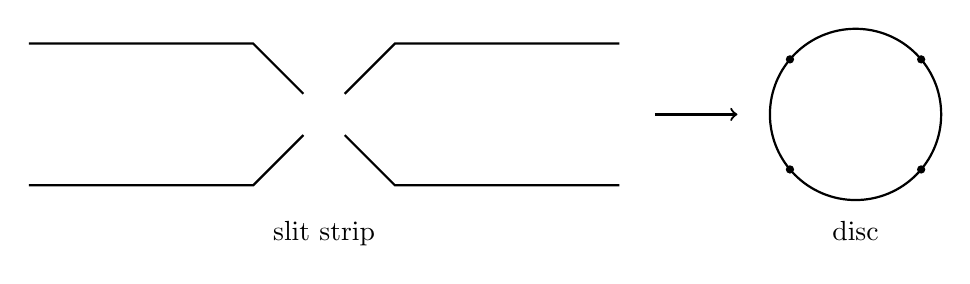
\begin{tikzpicture}[x=0.75cm,y=0.75cm]
    \draw[thick] (-5,1.2) -- (-1.2,1.2) -- (-0.35,0.35);
    \draw[thick] (-5,-1.2) -- (-1.2,-1.2) -- (-0.35,-0.35);
    \draw[thick] (0.35,0.35) -- (1.2,1.2) -- (5,1.2);
    \draw[thick] (0.35,-0.35) -- (1.2,-1.2) -- (5,-1.2);
    \draw[->,thick] (5.6,0) -- (7.0,0);
    \draw[thick] (9.0,0) circle (1.45);
    \foreach \a in {40,140,220,320} \fill (9.0,0) ++(\a:1.45) circle (1.5pt);
    \node[below] at (0,-1.65) {slit strip};
    \node[below] at (9.0,-1.65) {disc};
  \end{tikzpicture}
  \end{adjustbox}
  \caption{칠판에 그린 등위 곡선의 비교와 슬릿 띠를 원판으로 보내는 등각 사상의 개략도. 네 외부 끝점은 네 개의 특별한 경계점이 된다.}
  \lectureframe{01:04:46}
  \label{fig:l07-strip-to-disc}
\end{figure}

좌표를 바꾸어도 외부 상태가 사라지는 것은 아니다. 운동량, 입자 종류, 진동자 준위 정보를 네 예외점에 삽입해야 한다. 이 정보를 담는 형식적 대상이 꼭짓점 연산자다. 구체적인 구성은 뒤로 미루지만, 그 역할은 분명하다. 이 연산자는 균일한 세계면 경로 적분을 특정 산란 실험으로 바꾼다.

등각 변환을 이용해 원판의 경계점 세 개를 편리한 기준 위치로 옮기고 나면 실수 상대 위치 하나가 남는다. 순서가 정해진 네 경계점의 교차비로 이를 나타낼 수 있다. 이것은 앞서 슬릿 띠에서 썼던 수명 \(\tau_0\)에 대응하는 원판의 양이다.

\begin{figure}[H]
  \centering
  \includegraphics[width=0.62\textwidth]{lecture_07_figure_13.png}
  \caption{원판 경계 위의 삽입점 네 개. 등각 자유도를 사용하면 순서가 정해진 이 점들의 배치에서 실수 모듈러스 하나만 남는다.}
  \lectureframe{01:10:55}
  \label{fig:l07-four-points}
\end{figure}

따라서 수명 적분은 사라진 것이 아니다. 남은 모듈러스에 대한 적분으로 바뀌었다. 관례적인 좌표 \(0<z<1\)를 사용하면 네 점 열린 끈 적분은 앞선 강의에서 본 것과 같은 형태가 된다.
\begin{equation}
  \mathcal A(s,t)\propto
  \int_0^1 z^{-s-1}(1-z)^{-t-1}\,dz.
  \label{eq:l07-modulus-integral}
\end{equation}

\section{한 표면의 두 극한}

모듈라이 공간의 한쪽 끝에서는 들어오는 쌍과 관련된 두 삽입점이 서로 가까워진다. 슬릿 띠 좌표계에서는 결합과 분리 사이의 간격이 길다는 뜻이다. 직접 채널의 중간 끈이 오랫동안 전파된다. 다른 쪽 끝에서는 이웃한 다른 한 쌍의 점들이 서로 가까워진다. 이때 같은 표면을 교차 채널 교환으로 해석하는 것이 자연스럽다. 띠에서는 서로 무관해 보이는 이 두 설명이 하나의 원판 적분에서 서로 이웃한 경계 극한이다.

이전 강의에서 사용한 대부분 양수 부호 규약으로 돌아가면,
\begin{equation}
  -s=(k_1+k_2)^2,
  \qquad
  -t=(k_1+k_3)^2.
  \label{eq:l07-mandelstam}
\end{equation}
직접 채널 한계에서는 \(s\)에 극점들이 배열되고, 교차 채널 한계에서는 \(t\)에 극점들이 배열된다.
\editorialnote{강의 후반부에 칠판에서는 만델스탐 불변량에 약식 부호를 사용하면서 동시에 \(s\)을 양의 질량중심계 에너지 제곱으로 식별한다. 식 \eqref{eq:l07-mandelstam}은 강의 6에서 확립한 대부분 양수 부호 규약을 유지한다.}

\begin{figure}[H]
  \centering
  \includegraphics[width=0.62\textwidth]{lecture_07_figure_14.png}
  \caption{두 채널 도표. 한 방향에서는 오랫동안 전파되고, 교차 방향에서는 교환이 일어난다.}
  \lectureframe{01:19:27}
  \label{fig:l07-channel-diagrams}
\end{figure}

\begin{figure}[H]
  \centering
  \includegraphics[width=0.72\textwidth]{lecture_07_figure_15.png}
  \caption{칠판에서는 원판 모듈러스의 두 극한을 비교하며 \(s\)-채널과 \(t\)-채널의 운동량 짝짓기를 다시 살펴본다.}
  \lectureframe{01:19:40}
  \label{fig:l07-st-board}
\end{figure}

따라서 하나의 해석적 대상이 두 전개를 모두 제공한다.
\begin{equation}
  \mathcal A(s,t)=\mathcal A(t,s).
\end{equation}
이것이 채널 쌍대성이다. 공명 현상에 관한 초기 해석에서는 직접 채널 상태들의 합이 교차 채널 교환까지 담을 수 있다는 사실이 기적으로 여겨졌다. 유클리드 세계면에서는 등각 대칭이 두 설명이 같은 표면에 속하는 이유를 보여 준다. 역사적으로 베네치아노 진폭이 발견된 1969 직후 이 해석이 제시되었다.

\begin{classroomqa}
\audiencequestion{교차 방향에 해당하는 슬릿 띠 그림도 있나요? \lecturetimestamp{01:20:49}}
\lecturerresponse{있다. 다만 시간이라고 부르는 방향을 다르게 정해야 한다. 같은 유클리드 표면을 다른 외부 끝점 쌍이 먼 과거와 미래에 놓이도록 자를 수 있다. 바로 이 대안적인 단면화 때문에 하나의 세계면을 둘 이상의 채널로 해석할 수 있다.}
\end{classroomqa}

\begin{classroomqa}
\audiencequestion{끈들이 결합해 있는 시간은 결합 상수로 결정되나요? \lecturetimestamp{01:21:39}}
\lecturerresponse{정해진 수명이 선택되는 것은 아니다. 수명은 적분 변수이며 모든 값이 기여한다. 결합 상수는 결합과 분리---즉 붕괴의 세기---에 대한 가중치를 조절해 진폭에 곱으로 들어간다. 모듈러스 적분을 대신하지는 않는다.}
\end{classroomqa}